\subsection{Когомологически тривиальные модули и теорема Тейта}

	Пусть $L/K$~--- расширение Галуа с группой Галуа $G$, $H \subset G$. Сейчас мы  построим следующую коммутативную диаграмму  (слева она, справа её когомологическая интерпретация):
	\begin{center}
			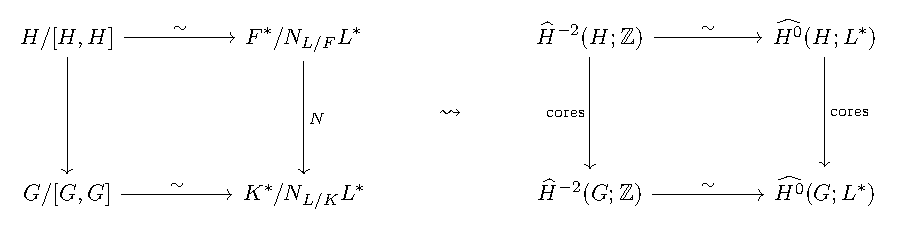
\includegraphics{lectures/6/pictures/cd_33.pdf}
	\end{center}

	Для этого нам понадобится следующее понятие: 

	\begin{definition} 
		Пусть $G$~--- конечная группа, $A \in G\text{-}\Mod$. $A$ называется \emph{когомологически тривиальным}, если $\forall H \subset F, \ \forall n \in \Z \ \widehat{H}^n(H, A) = 0$. 
	\end{definition}

	\begin{statement}\label{cohomology_trivial_criterion} 
		Пусть $\exists n \ge 0 \colon \forall H \subset G \ \widehat{H}^n(H; A) = \widehat{H}^{n + 1}(H; A) = 0$. Тогда модуль $A$ когомологически тривиален. 
	\end{statement}
	\begin{proof}
		\bf{Шаг 1:} докажем это утверждение, когда $G$~--- $p$-группа.

		 Будем вести индукцию по $|G|$, база очевидна. 

		 Выберем нормальную подгруппу $H$ индекса $p$. Так как $|H| \le |G|$, по индукционному предположению $A$ является когомологически тривиальным $H$-модулем. 

		 Рассмотрим сначала отдельно случай, когда $n \ge 0$. Тогда (в силу того, что $H^1(H, A) = \ldots = H^{n - 1}(H, A) = 0$) мы можем записать точную последовательность для ограничения и инфляции: 
		\begin{center}
			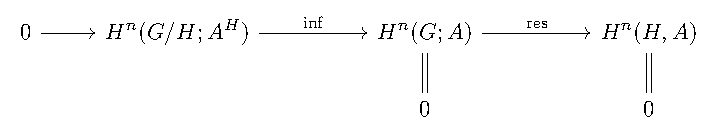
\includegraphics{lectures/6/pictures/cd_34.pdf}
		\end{center}
		из которой мы заключаем, что $H^n(G/H, A^H) = 0$. Аналогично мы понимаем, что $H^{n + 1}(G/H, A^H) = 0$

		 Группа $G/H$ циклическая, а значит, в силу периодичности, из того, что зануляются две соседних группы когомологий следует, что зануляются все группы когомологий, то есть $\widehat{H}^i(G/H, A^H) = 0$, то есть $A^H$~--- когомологически тривиальный $G/H$-модуль (так как $G/H$~--- циклическая группа порядка $p$ и нетривиальных подгрупп у неё просто нет).  
		
		Теперь пусть $n = 0$. Тогда 
		\[
			\widehat{H}^0(G/H; A^H) = (A^H)^{G/H}/N_{G/H}A^H.
		\]
		С другой стороны, мы знаем, что $0 = \widehat{H}^0(G; A) = A^G/N_G A$, и, кроме того, выполнено равенство $(A^H)^{G/H} = A^G$. Кроме того, $N_{G/H}A^H \supset N_G A$, так как 
		\[
			G = \bigsqcup \sigma_i H \implies Na = \sum_{g \in G} g a = \sum_{\sigma_i \in G/H} \sigma_i \underbrace{\lr*{\sum_{h \in H} (ha)}}_{\in A^H},
		\]
		откуда одна группа~--- фактор другой, откуда $\widehat{H}^0(G/H; A^H) = 0$, то есть $A^H$~--- когомологически тривиальный $G/H$-модуль. 

		Осталось доказать, что что $\widehat{H}^i(G; A) = 0 \ \forall i$. 

		В случае $i \ge 1$ мы получаем это из точной последовательности для ограничения и инфляции: 

		\begin{center}
	       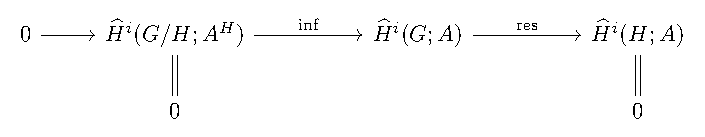
\includegraphics{lectures/6/pictures/cd_35.pdf},
		\end{center}
		так как выше мы показали, что $A^H$~--- когомологически тривиальный $G/H$-модуль, а по индукционному предположению $A$~--- когомологически тривиальный $H$-модуль. 


	Теперь разберём случай  $i \le 1$. Запишем длинную точную последовательность когомологий, связанную с короткой точной последовательностью 
	\[
		0 \to B \to A_* \to A \to 0.
	\]
	При помощи связывающего гомоморфизма из неё мы получим $\widehat{H}^{m + 1}(G, B) = \widehat{H}^m(G, A)$.

	Тогда по доказанному для $i \ge 1$ мы получаем, что $H^{i}(G, B) = 0$. В частности, $\widehat{H}^1(G; B) = 0$, но 
	\[
		\widehat{H}^0(G, A) = \widehat{H}^1(G, B) = 0.
	\]
	Так мы можем и дальше сдвигать размерности и получать, что 
	\[
		\widehat{H}^{-1}(G; A) = \widehat{H}^0(G; B) = 0
	\]
	и так далее. Итак, мы полностью закончили первый шаг доказательства. 

	\noindent\bf{Шаг 2:} пусть $G$~--- произвольная группа. Тогда мы поступим также, как и в ugly-lemma: отображение
	\begin{center}
			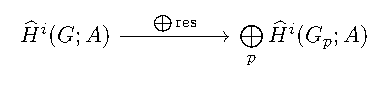
\includegraphics{lectures/6/pictures/cd_36.pdf}
	\end{center}
	является мономорфизмом, а каждое слагаемое справа когомологически тривиально по первому шагу доказательства. 
	\end{proof}

	\begin{remark}
		Из рассуждения со сдвигом размерности видно, что требование $n \ge 0$ в теореме не по существу. 
	\end{remark}

    Теперь двинемся дальше. Пусть $A \in G\text{-}\Mod$, зададимся следующим вопросом: \emph{когда существует система изоморфизмов $\widehat{H}^n(H; \Z) \xrightarrow{\sim} \widehat{H}^n(H; A)$, индуцированная некоторым морфизмом $G$-модулей $\Z \to A$?}

	Получим необходимое условие существования такой системы для всех $H \subset G$ и $n \in \Z$. Предположим сначала, что 
	\[
		\widehat{H}^{-1}(H; \Z) \cong \widehat{H}^{-1}(H; A), \text{ но } \widehat{H}^{-1}(H; A) = \Ker{N}/\langle \sigma - 1 \rangle A,
	\]

	Соответственно,  так как $\Z$~--- тривиальный $\Z$-модуль, уже $N(a) = |G|a = 0 \implies a = 0$, октуда $\Ker{N} = 0$ и группа $\widehat{H}^{-1}(H; \Z)$ будет нулевой. 

	Теперь, пусть у нас есть последовательность подгрупп $P \subset H \subset G$. Тогда у нас есть соответствующая коммутативная диаграмма (и её частный случай для $n = 0$):
	\begin{center}
		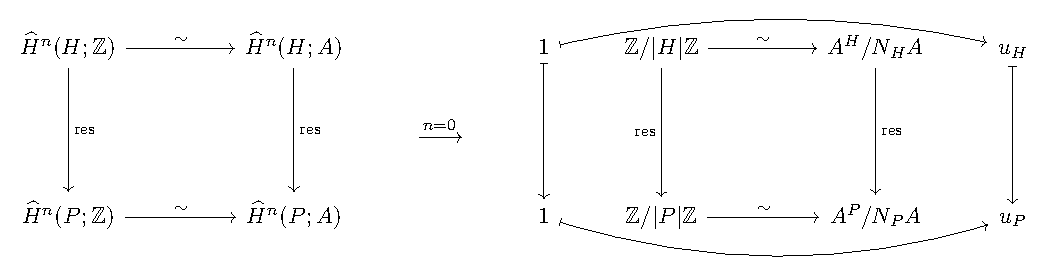
\includegraphics{lectures/6/pictures/cd_37.pdf}
	\end{center}

	То есть, нам нужно, чтоб группы $A^H/N_{H}A $ были цикличны и имели порядок $|H|$ для всех подгрупп $|H|$, и кроме того, существовали образующие $u_H$ такие, что $\mathrm{res}_{H/P}(u_H) = u_{P}$.

	Еще это условие можно переформулировать таким образом: в $A^G/N_G A$ можно выбрать образующую $u_{G}$ так, что $\res(u_G) = u_H$. Итого, мы получили два необходимых условия: 

	\begin{enumerate}
		\item $\widehat{H}^{-1}(H, 0) = 0$.

		\item В $A^G/N_G A$ можно выбрать образующую $u_{G}$ так, что $\res(u_G) = u_H$
	\end{enumerate}

	\begin{theorem}[Тейт] 
		Эти условия являются достаточными.
	\end{theorem}
	\begin{proof}
		Итак, рассмотрим наш гомоморфизм, $\Z \to A$, он переводит 1 в прообраз $u_{G}$ при факотризации. 

		Рассмотрим короткую точную последовательность
		\[
			 0 \to X \to A_* \oplus \Z \to A \to 0,
		\]
		Покажем, что $X$ когомологически тривиален, пользуясь предложением~\ref{cohomology_trivial_criterion}. А конкретнее, покажем, что 
		\[
		 	\forall H \le G \quad \widehat{H}^0(H, X) = \widehat{H}^1(H, X) = 0.
		 \] 

		Запишем длинную точную последовательность когомологий: 
		\begin{center}
			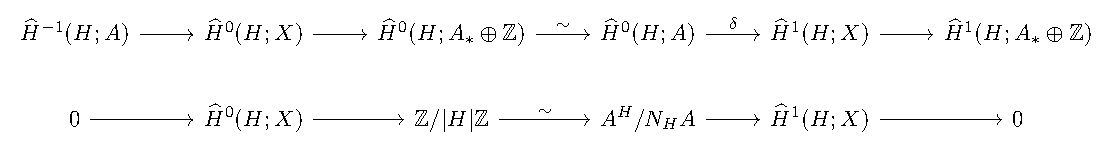
\includegraphics[scale = 0.9]{lectures/6/pictures/cd_38.pdf}
	\end{center}
		Поясним, почему на ней всё устроено именно так. 

		\begin{itemize}
			\item $H^{-1}(H, A) = 0$ по первому условию. 

			\item $\widehat{H}^0(H, A_* \oplus \Z) \cong \widehat{H}^0(H, A_*) \oplus \widehat{H}^0(H,\Z) \cong \widehat{H}^0(H,\Z) \cong \Z/|H|\Z$.

			\item В силу условия 2 у нас есть вот такая коммутативная диаграмма: 

			\begin{center}
				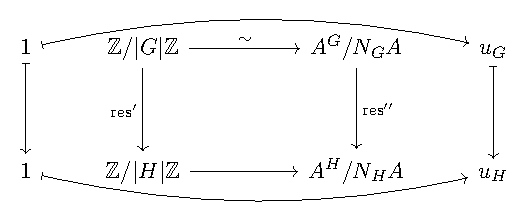
\includegraphics{lectures/6/pictures/cd_43.pdf}
			\end{center}

			Так как $\res''$ сюръективен, $\Z/|H|\Z \twoheadrightarrow A^H/N_H A$, но порядок этих групп совпадает и равен $|H|$, откуда мы понимаем, что 
			\[
				\widehat{H}^0(H, A_* \oplus \Z) \cong \Z/|H|\Z \cong A^H/N_H A \cong \widehat{H}^0(H, A).
			\]

			\item $\widehat{H}^1(H, A_* \oplus \Z) \cong \widehat{H}^{1}(H, A_*) \oplus \widehat{H}^{1}(H, \Z) \cong \Hom(H, \Z) = 0$. 
		\end{itemize}

		Тогда из длинной точной последовательности, написанной выше мы видим, что $\forall H \le G \quad \widehat{H}^0(H, X) = \widehat{H}^1(H, X) = 0$, а значит, по предложению~\ref{cohomology_trivial_criterion} $X$~--- когомологически тривиальный $G$-модуль. Тогда вновь из длинной точной последовательности когомологий мы получаем, что 
		\[
			\widehat{H}^{n}(H, A_* \oplus \Z) \xrightarrow{\sim} \widehat{H}^n(H, A),
		\]
		но $\widehat{H}^{n}(H, A_* \oplus \Z) \cong \widehat{H}^{n}(H, \Z)$, так что мы получили, что хотели. 
 	\end{proof}

 	\begin{corollary}[Тейт]
 		Пусть $A \in G-\Mod$. Предположим, что выполнены следующие условия 
 		\begin{enumerate}
 			\item Для любой подгруппы $H \subset G$ мы имеем $H^1(H, A) = 0$.

 			\item Для любой подгруппы $H \subset G$ группа $H^2(H, A)$~--- циклическая группа порядка $|H|$.

 			\item $\res_{H/P}{u_{H}} = u_{P}$ для любой подгруппы $P \subset H$. 	
 		\end{enumerate}

 		Тогда существует система изоморфизмов $H^n(H; A) \to H^{n - 2}(H; \Z)$, причем эти изоморфизмы согласованы с ограничениями и коограничениями, то есть, следующие диаграммы коммутативны: 
 		\begin{center}
				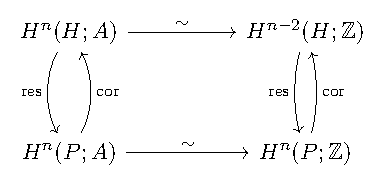
\includegraphics[scale = 0.9]{lectures/6/pictures/cd_39.pdf}
	\end{center}

 	\end{corollary}
 	\begin{proof}
 		
 		Запишем следующие короткие точные последовательности 
 		\[
 			0 \to A \to A^* \to A' \to 0
 		\]
 		\[
 			0 \to A' \to (A')^* \to (A')' \to 0
 		\]
 		Так как модуль по центру коиндуцированный, мы получаем, что 
 		\[
 			H^{n - 2}(H; A'') \cong H^{n - 1}(H; A') \cong H^n(H; A).
 		\]

 		Применяя теорему Тейта для $A''$ мы получаем нужное:
 		\[
 			H^{n}(H; A) \cong \widehat{H}^{n - 2}(H, (A')') \cong H^{n - 2}(H; \mathbb{Z}),
 		\]
 		чего мы собственно и хотели. 
 	\end{proof}

 		Возьмём $G = \Gal(L/K)$, $A = L^*$, тогда как мы помним, группа $H^2(H, L^*)$~--- циклическая группа порядка $|H|$, то есть условие $1$ выполнено. Условие $2$ следует из приведённой ранее коммутативной диаграммы для группы Брауэра. Тогда, применяя следствие, мы получаем, в частности, что 

   \[ H^n(G; L^*) \cong H^{n - 2}(G; \mathbb{Z}) ,\] 
   а в частности 
 	\[
 		 \implies \widehat{H}^{0}(G; L^*) = F^* /N_{L/F}L^* \cong G/[G, G] = \widehat{H}^{-2}(G; \Z).
 	\]

    \begin{corollary}\label{normal_subgroup_abelinisation}
 		Пусть $L/K$~--- конечное расширение локального поля $K$ с группой Галуа $G$. Тогда 
 		\[	
 		 K^*/N_{L/K}L^* \cong G^{ab}
 		 \]
 	\end{corollary}